\chapter{Granularity}
\label{chap:granularity}
As described in Chapter~\ref{chap:prelim}, a transition relation is considered to be a conjunction of Boolean formulas. The granularity of these formulas will substantially affect the analysis results. Depending on how contracts are specified in the model, it is possible to have a ``complete" specification, i.e., all of the equations in the model are required to determine the validity of the property. However, in certain cases, subexpressions of equations may be irrelevant. If the equation is decomposed into smaller pieces, this incompleteness becomes visible and the model is no longer completely covered.\footnote{Simply put, coverage is a metric that determines how well properties cover the design of a model.} It is often the case that splitting an equation of the model into more conjuncts, or equivalently, making the model more \textit{granular}, leads to lower coverage of the model. This would be reflected in the IVCs generated for a given safety property; the IVCs in a more granular model would theoretically reflect only the necessary equations required for property verification, and thus would provide more specific analysis results.

Granularity has been previously discussed by Ghassabani~\cite{ghassabani_2018}, but to our knowledge has not been discussed in any other previous work -- in particular related to minimal cut set generation. Since IVC generation is a required first step of our minimal cut set algorithms, it is important to discuss how the granularity of the model will affect the cut sets generated through this approach. 

As described in Chapter~\ref{chap:mcsGen}, the backend model checker used in this transformation is \jkind which performs $k$-induction over a transition system defined with a Lustre program. Ghassabani did a preliminary investigation of granularity within the context of the Lustre language which provides a nice formalism for this discussion because it is top-level conjunctive, equational, and \textit{referentially transparent}~\cite{Halbwachs91:IEEE}. This means that the behavior of a Lustre program is defined by a system of equations and any subexpression on the right side of an equation can be extracted and assigned a fresh variable\footnote{A fresh variable is a variable with an identifier that has not been used within the program.} which is substituted into the original equation without changing the meaning of the program. In this context, \textit{granular refinement} is defined as an extraction of a subexpression into a new equation assigning a fresh variable. 

\section{Illustrative Example of Granularity}
To see how different representations of the system will alter the IVC and MinCutSet computations, let us examine a simple sensor example system built by engineer A. The top level safety property states: 
\begin{center}
    \textit{If environmental temperature reaches 90 degrees, then system reports high temperature.}
\end{center}

The direct subcomponent is the temperature sensor system which contains two outputs: (1) a high temp indicator, and (2) the actual temperature. Engineer A chose to write the supporting contract in the temperature subsystem as follows: 
\begin{center}
    $(T \geq 90 \implies temp\_high) \land (temp\_indicator = T)$ 
\end{center}
  
The example temp sensor system is shown in Figure~\ref{fig:granularityEx1}.  

\begin{figure}[h]
\begin{center}
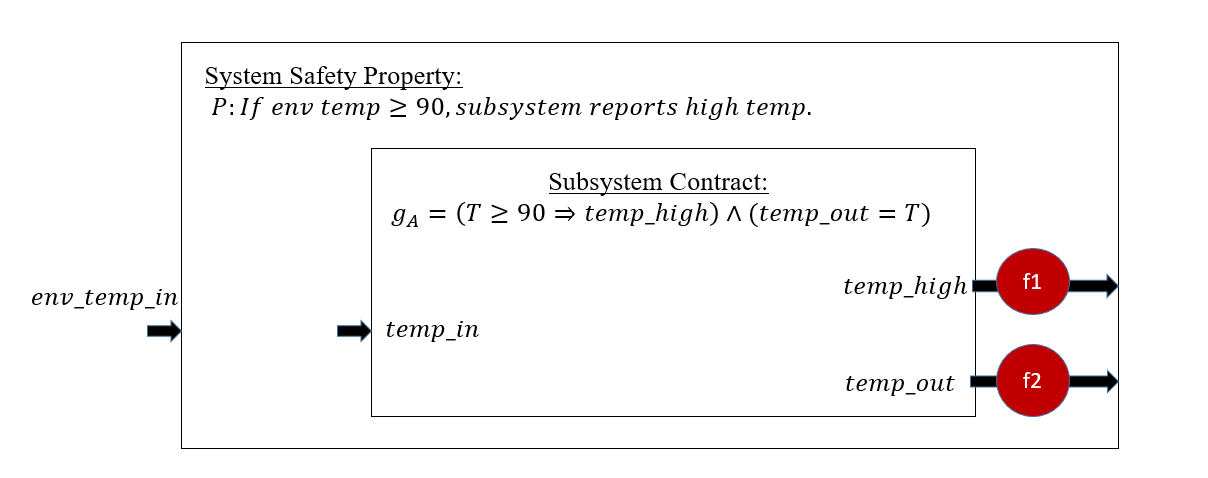
\includegraphics[width=14cm]{images/granularityEx1.PNG}
\caption{Temp Sensor System Contract Part I} \label{fig:granularityEx1}
\end{center}
\end{figure}

The safety property at the top level requires the contract $g_A$ for proof of validity. Thus, the \aivcalg will contain the contract $g_A$ as an IVC. 

There are two faults defined for the temperature subsystem; one for each of the outputs. Fault $f_1$ affects the $temp\_high$ output and fault $f_2$ affects the $temp\_out$ output. Since each of these faults will violate the contract $g_A$, each of them will be found in the \textit{MinCutSets} for $G_A$.

Now assume that Figure~\ref{fig:granularityEx2} was the system representation built by engineer B. 

\begin{figure}[h]
\begin{center}
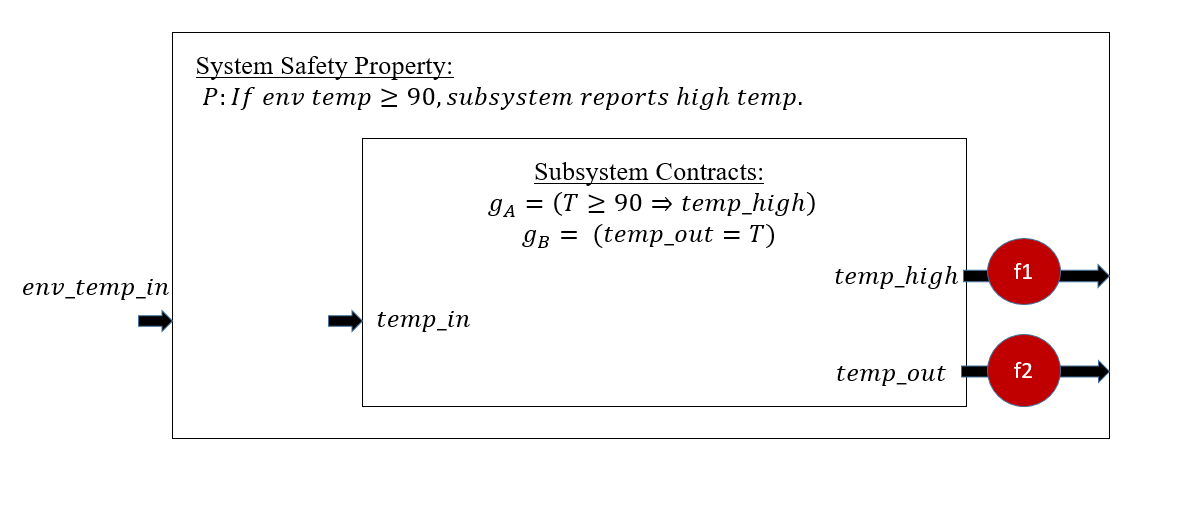
\includegraphics[width=14cm]{images/granularityEx2.PNG}
\caption{Temp Sensor System Contract Part II} \label{fig:granularityEx2}
\end{center}
\end{figure} 

The behavior and architecture of the system is the same, but the contract for the subsystem is more \textit{granular}; it is stated as two separate contracts:
\begin{center}
    $ g_A = (T \geq 90 \implies temp\_high)$ \\ 
    $ g_B = (temp\_indicator = T)$ 
\end{center}

Since $g_B$ is not required for the proof of the system safety property, only $g_A$ is found in the \textit{IVC}s and thus only $f_1$ will be seen in the \textit{MinCutSets} for this particular contract. 

In this simple example, it is easy to see how the granularity of the contracts may greatly affect the results of analysis.

\section{Algorithms and Testing Results}
